%\documentclass[iop,revtex4]{emulateapj}% change onecolumn to iop for fancy, iop to twocolumn for manuscript
\documentclass[twocolumn]{emulateapj}% change onecolumn to iop for fancy, iop to onecolumn for manuscript
%\documentclass[12pt,preprint]{aastex}

\usepackage{graphicx}
\usepackage[caption=false]{subfig}
%\usepackage{lineno}
%\usepackage{blindtext}
%\linenumbers
%\usepackage{breqn}
\usepackage{amsmath}

\let\pwiflocal=\iffalse \let\pwifjournal=\iffalse
%From: http://arxiv.org/format/1512.00483
%\input{setup}
\usepackage{enumerate}
\usepackage{amsmath,amssymb}
\usepackage{bm}
\usepackage{color}
\usepackage[utf8]{inputenc}

%% For anyone who downloaded my source file from arxiv:
%% I stole most of this setup.tex from a paper by Peter .K.G. Williams, but I made a bunch of edits to satisfy my own needs. You might check his paper out (http://arxiv.org/abs/1409.4411) for the original source file or contact him if you have any questions, since I don't really understand how some of these things work. 
%One cool thing it does is you can define an object, just that when someone clicks on the pdf it will link to simbad. I could never quite get this to work, probably because you have to get the text exactly right and my motivation for getting it to work was not super high. 


% basic packages
\usepackage{amsmath,amssymb}
\usepackage[breaklinks,colorlinks,urlcolor=blue,citecolor=blue,linkcolor=blue]{hyperref}
\usepackage{epsfig}    
\usepackage{graphicx}    
\usepackage{lineno}
\usepackage{natbib}
\usepackage{bigints}
\usepackage[outdir=./]{epstopdf}



% font stuff
\usepackage[T1]{fontenc}
\pwifjournal\else
  \usepackage{microtype}
\fi


% emulateapj has overly conservative figure widths, I think because some
% people's figures don't have good margins. Override.
\pwifjournal\else
  \makeatletter
  \renewcommand\plotone[1]{%
    \centering \leavevmode \setlength{\plot@width}{0.95\linewidth}
    \includegraphics[width={\eps@scaling\plot@width}]{#1}%
  }%
  \makeatother
\fi


\makeatletter

\newcommand\@simpfx{http://simbad.u-strasbg.fr/simbad/sim-id?Ident=}

\newcommand\MakeObj[4][\@empty]{% [shortname]{ident}{url-escaped}{formalname}
  \pwifjournal%
    \expandafter\newcommand\csname pkgwobj@c@#2\endcsname[1]{\protect\object[#4]{##1}}%
  \else%
    \expandafter\newcommand\csname pkgwobj@c@#2\endcsname[1]{\href{\@simpfx #3}{##1}}%
  \fi%
  \expandafter\newcommand\csname pkgwobj@f#2\endcsname{#4}%
  \ifx\@empty#1%
    \expandafter\newcommand\csname pkgwobj@s#2\endcsname{#4}%
  \else%
    \expandafter\newcommand\csname pkgwobj@s#2\endcsname{#1}%
  \fi}%

\newcommand\MakeTrunc[2]{% {ident}{truncname}
  \expandafter\newcommand\csname pkgwobj@t#1\endcsname{#2}}%

\newcommand{\obj}[1]{%
  \expandafter\ifx\csname pkgwobj@c@#1\endcsname\relax%
    \textbf{[unknown object!]}%
  \else%
    \csname pkgwobj@c@#1\endcsname{\csname pkgwobj@s#1\endcsname}%
  \fi}
\newcommand{\objf}[1]{%
  \expandafter\ifx\csname pkgwobj@c@#1\endcsname\relax%
    \textbf{[unknown object!]}%
  \else%
    \csname pkgwobj@c@#1\endcsname{\csname pkgwobj@f#1\endcsname}%
  \fi}
\newcommand{\objt}[1]{%
  \expandafter\ifx\csname pkgwobj@c@#1\endcsname\relax%
    \textbf{[unknown object!]}%
  \else%
    \csname pkgwobj@c@#1\endcsname{\csname pkgwobj@t#1\endcsname}%
  \fi}

\makeatother


% Evil magic to patch natbib to only highlight the year paper refs, not the
% authors too; as seen in ApJ. From
% http://tex.stackexchange.com/questions/23227/.

\pwifjournal\else
  \usepackage{etoolbox}
  \makeatletter
  \patchcmd{\NAT@citex}
    {\@citea\NAT@hyper@{%
       \NAT@nmfmt{\NAT@nm}%
       \hyper@natlinkbreak{\NAT@aysep\NAT@spacechar}{\@citeb\@extra@b@citeb}%
       \NAT@date}}
    {\@citea\NAT@nmfmt{\NAT@nm}%
     \NAT@aysep\NAT@spacechar\NAT@hyper@{\NAT@date}}{}{}
  \patchcmd{\NAT@citex}
    {\@citea\NAT@hyper@{%
       \NAT@nmfmt{\NAT@nm}%
       \hyper@natlinkbreak{\NAT@spacechar\NAT@@open\if*#1*\else#1\NAT@spacechar\fi}%
         {\@citeb\@extra@b@citeb}%
       \NAT@date}}
    {\@citea\NAT@nmfmt{\NAT@nm}%
     \NAT@spacechar\NAT@@open\if*#1*\else#1\NAT@spacechar\fi\NAT@hyper@{\NAT@date}}
    {}{}
  \makeatother
\fi

\newcommand{\prob}{{\rm prob}}
\newcommand{\qN}{\{q_i\}_{i=1}^N}
\newcommand{\qM}{\{q_{im}\}_{i=1,m=0}^{N,M}}
\newcommand{\yN}{\{y_i\}_{i=1}^N}

\newcommand{\kms}{ \textrm{km s}^{-1} }

\newcommand{\vM}{\mathsf{M}}
\newcommand{\vD}{\mathsf{D}}
\newcommand{\vR}{\mathsf{R}}
\newcommand{\vC}{\mathsf{C}}
\newcommand{\fM}{ \vec{{\bm M}}}
\newcommand{\fMi}{M_i}
\newcommand{\fD}{ \vec{{\bm D}}}
\newcommand{\fDi}{D_i}
\newcommand{\fR}{ {\bm R}}
\newcommand{\dd}{\,{\rm d}}
\newcommand{\trans}{\mathsf{T}}
\newcommand{\teff}{T_\textrm{eff}}
\newcommand{\teffa}{T_\textrm{amb}}
\newcommand{\teffb}{T_\textrm{spot}}
\newcommand{\logg}{\log g}
\newcommand{\Z}{[{\rm Fe}/{\rm H}]}
\newcommand{\A}{[\alpha/{\rm Fe}]}
\newcommand{\vsini}{v \sin i}
\newcommand{\matern}{Mat\'{e}rn}
\newcommand{\HK}{$\textrm{H}_2$O-K2}
\newcommand{\cc}[2]{c_{#2}^{(#1)}} 

\newcommand{\flam}{f_\lambda}
\newcommand{\vt}{ {\bm \theta}}
\newcommand{\vT}{ {\bm \Theta}}
\newcommand{\vp}{ {\bm \phi}}
\newcommand{\vP}{ {\bm \Phi}}
\newcommand{\cheb}{ \vp_{\mathsf{P}}}
\newcommand{\chebi}[1]{ \vp_{\textrm{Cheb}_{#1}}}
\newcommand{\Cheb}{ \vP_{\textrm{Cheb}}}
\newcommand{\Chebi}[1]{ \vP_{\textrm{Cheb}_{\ne #1}}} 
\newcommand{\cov}{ \vp_{\mathsf{C}}}
\newcommand{\covi}[1]{ \vp_{\textrm{cov}_{#1}}} 
\newcommand{\Cov}{ \vP_{\textrm{cov}}}
\newcommand{\Covi}[1]{ \vP_{\textrm{cov}_{\ne #1}}} 

\newcommand{\allParameters}{\vT} 
\newcommand{\nuisanceParameters}{\vP} 

\newcommand{\KK}{\mathcal{K}}
\newcommand{\Kglobal}{\KK^{\textrm{G}}}
\newcommand{\Klocal}{\KK^{\textrm{L}}}

\newcommand{\Gl}{Gl\,51}
\newcommand{\PHOENIX}{{\sc Phoenix}}

% Appendix commands
\newcommand{\wg}{\mathbf{w}^\textrm{grid}}
\newcommand{\wgh}{\hat{\mathbf{w}}^\textrm{grid}}

\newcommand{\Sg}{\mathbf{\Sigma}^\textrm{grid}}


\newcommand{\todo}[1]{ \textcolor{blue}{\\TODO: #1}}
\newcommand{\comm}[1]{ \textcolor{red}{MGS: #1}}
\newcommand{\hili}[1]{ \textcolor{green}{#1}}
\newcommand{\ctext}[1]{ \textcolor{blue}{\% #1}}


%  From Peter Williams and Andy Mann again:
\newcommand{\um}{$\mu$m}


\newcommand{\iancze}{{\sc C15}}

\providecommand{\eprint}[1]{\href{http://arxiv.org/abs/#1}{#1}}
\providecommand{\adsurl}[1]{\href{#1}{ADS}}
\newcommand{\name}{LkCa 4 }
\newcommand{\project}[1]{\textsl{#1}}
%\def\vsini{$v\sin{i_*}$}

\slugcomment{In preparation}

\shorttitle{Spots on Sub-subgiants}

\shortauthors{TBD}

\bibliographystyle{yahapj}

\begin{document}

\title{Starspots on sub sub giants }

\author{TBD,\altaffilmark{1}, author list TBD}


\altaffiltext{1}{TBD}

\begin{abstract}

We measure the starspots on a sub sub giant.

\end{abstract}

\keywords{stars: fundamental parameters ---  stars: statistics}

\maketitle

\section{Introduction}\label{sec:intro}

Sub-subgiant stars are stars that lie below the subgiant branch on a cluster optical color-magnitude diagram (CMD), but are too red to be main sequence stars. These stars are commonly found in evolved open clusters and globular clusters, with 65 sub-subgiants currently identified across 17 different clusters \citep{geller17}. The majority of sub-subgiant stars are single-lined spectroscopic binaries with short orbital periods of a few days with moderate X-ray luminosities of $10^{30}$ to $10^{31}$ erg s$^{-1}$ \citep[and references therein]{geller17}.

The presence of sub-subgiants cannot be explained with typical single-star stellar evolutionary pathways. Three possible formation scenarios for sub-subgiants were put forth by \citet{leiner17}: mass transfer in a binary system, stripping of a subgiant star envelope through a dynamical encounter, and reduced luminosity as a result of inhibited convection due to the presence of strong magnetic fields. \citet{leiner17} conclude that strong magnetic fields due to binary interactions would produce the largest number of sub-subgiants.

In this paper we focus on a single sub-subgiant system, S1063 in the open cluster M67. This system is a prototypical sub-subgiant star, with an single-lined spectroscopic orbital period of 18.4 days \citep{geller17}, an X-ray luminosity of $1.3\times10^{31}$ erg s$^{-1}$ \citep{vandenberg99}, and a variable light curve in \textit{K2} (REF LIGHT CURVE SECTION?).

\subsection{Starspots as confounding factors}
Mass, age, and metallicity uniquely map a main sequence star to its HR diagram position.  A fourth factor---rotation---confounds this mapping in as-yet-unknown ways.  Rotation might enhance spread in HR diagram positions (cite XX Davenport, Douglas?), with the most conspicuous spreads in the pre-main sequence regime (cite XX Covey, Stauffer).  Spreads in the HR diagram offer clues to the consequences of rotation.  Increased rotation heightens the magnetic dynamo strength and concommitant surface magnetic field.  These magnetic fields suppress convective efficiency, meaning the star must increase in size at a lower effective temperature to allow the same amount of internal energy to escape (cite XX Feiden): rotating stars become bigger and cooler than their non-rotating counterparts (cite XX Somers).  The interplay of rotation, dynamo, and surface fields remain an active area of research, with bright prospects for a unified theory involving the degree of magnetic complexity parameter (cite XX Garraffo).

Surface magnetic fields offer two key observational manifestations.  The Zeeman Effect splits spectral line levels in magnetic-sensitive atomic transitions (cite XX Johns-Krull).  Starspots induce stellar surface inhomogeneities that can be seen in the modulation of

The story in the post-main sequence is less clear.  Angular momentum transport governs rotation  as stars evolve over orders of magnitude in size.


%Fill in more theory here
\citet{somers15} emphasized the roll of starspots in inferring stellar ages.

\begin{itemize}
\item What is a sub-subgiant?
  \begin{itemize}
  \item What causes sub sub giant stars (Leiner et al. 2017)
  \end{itemize}
\item M67 S1063
\begin{itemize}
  \item Prototypical subsub (Geller et al. 2017)
  \item Binary orbit, SB1
\end{itemize}
\item Starspots as confounding factors
\begin{itemize}
  \item Inhibit convective efficiency (redder and bigger)
  \item Also confound observations: assign incorrect Teff
  \item This paper aims to measure the starspot coverage and temp
\end{itemize}
\item Layout of this paper
\end{itemize}

\section{Observation and data reduction}
\subsection{IGRINS observations}
A high resolution spectrum of S1063 was acquired with the $R=45,000$ Immersion Grating Infrared Spectrograph \citep[IGRINS;][]{park14} at UT 2015-04-26 $03^h29^m$ at the $2.7\;$m Harlan J. Smith Telescope at McDonald Observatory.  Eight 600-second individual exposures were acquired in an ABBA nod pattern at an airmass of 1.2.  The sky emission lines and telluric lines were removed with the IGRINS Pipeline Package  \citep[PLP;][]{jaejoonlee16} and a reference A0V star acquired nearby in time and airmass.
The $H-$band spectra exhibited signal-to-noise ratio $S/N\sim30-80$ per pixel (\textbf{verify XX}).
The $K-$band spectra possessed low $S/N$ and were excluded from further analysis.

\begin{figure*}[hbt!]
  \centering
  \begin{tabular}{ccccc}
    \subfloat{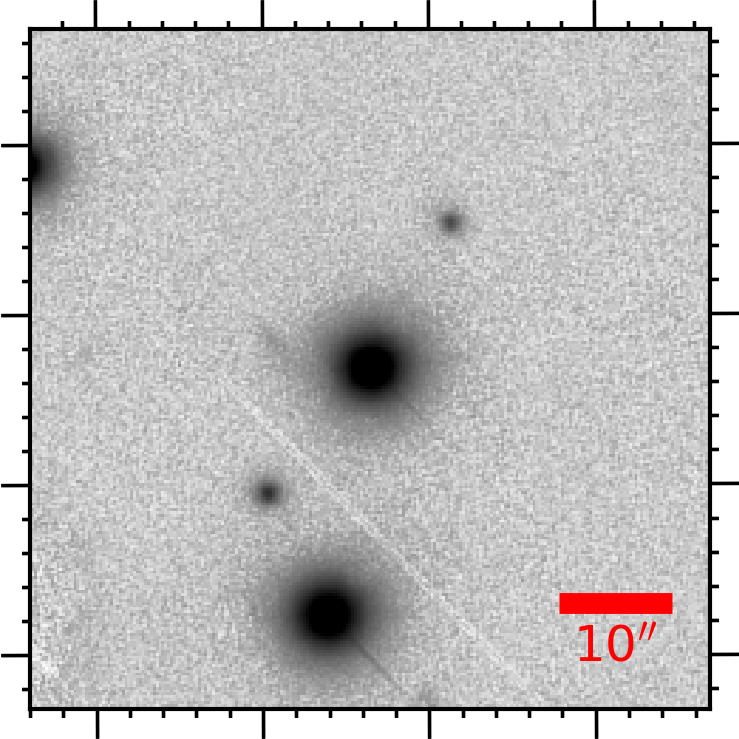
\includegraphics[width=1in]{figures/S1063_60x60arcsec_PS1_g.png}} &
    \subfloat{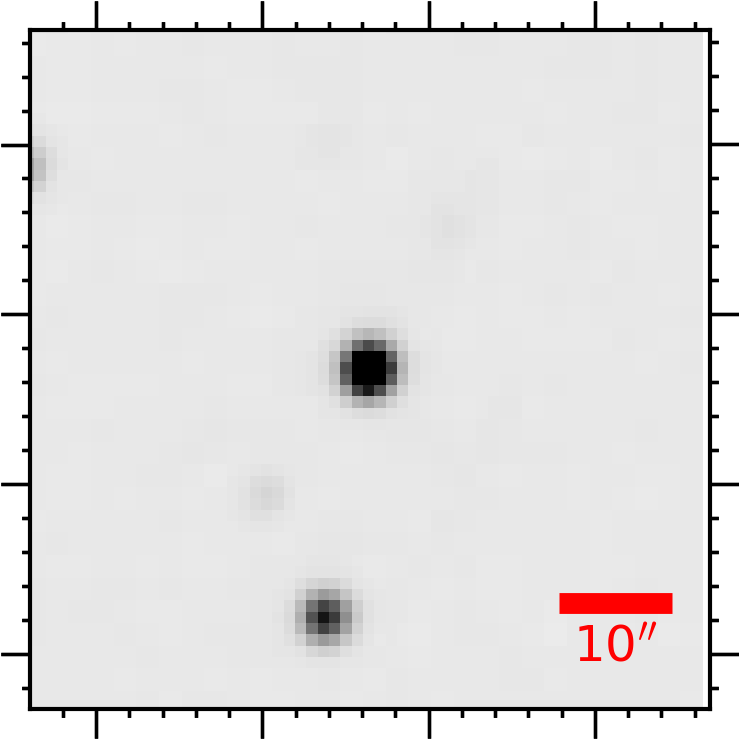
\includegraphics[width=1in]{figures/S1063_60x60arcsec_2M_J.png}} &
    \subfloat{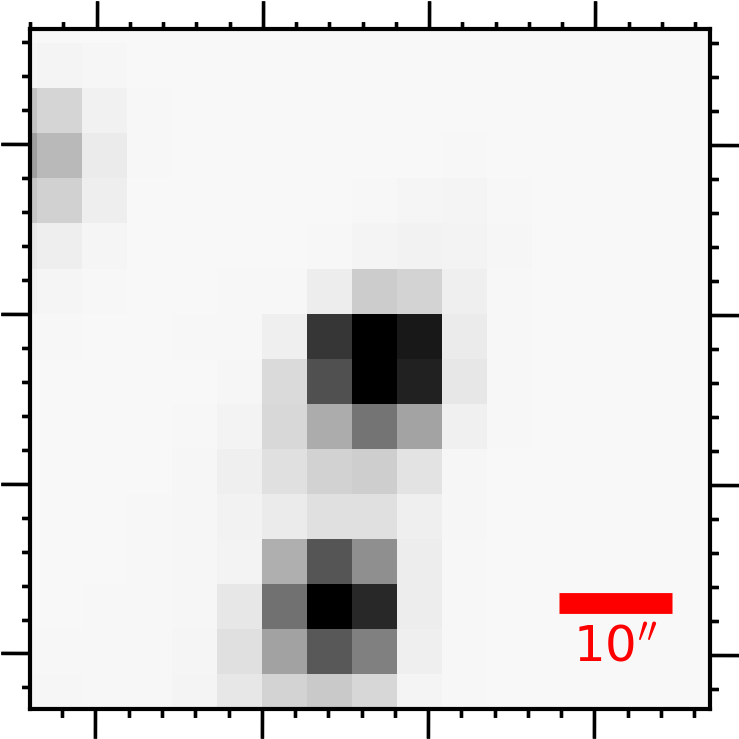
\includegraphics[width=1in]{figures/S1063_60x60arcsec_K2_C5.png}} &
    \subfloat{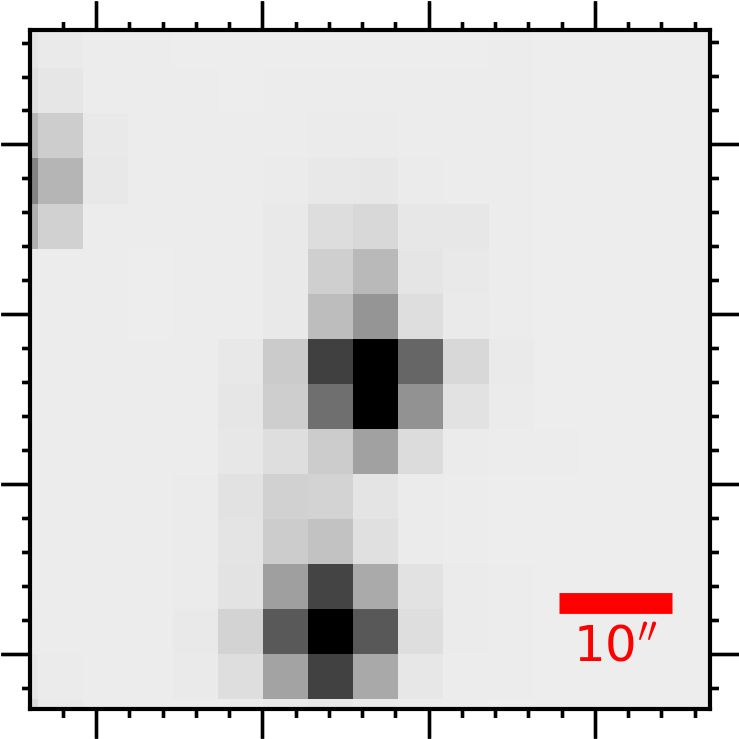
\includegraphics[width=1in]{figures/S1063_60x60arcsec_K2_C16.png}} &
    \subfloat{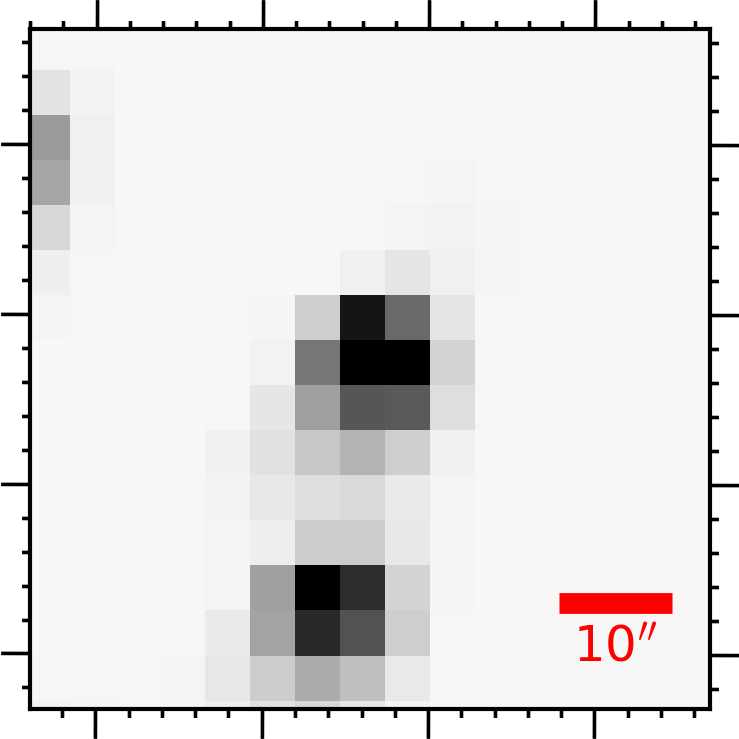
\includegraphics[width=1in]{figures/S1063_60x60arcsec_K2_C18.png}} \\
  \end{tabular}
\caption{Imaging of S1063 in $60'' \times 60''$ postage stamps. \emph{left-to-right:} Pan-STARRS $g$-band co-added image contemporaneous with C16; 2MASS $J-$band; K2 Campaigns 5, 16, 18 from Full Frame Images.  S1063 is sufficiently separated from nearby sources in the coarse \emph{Kepler} imaging.}
\label{fig:imaging}
\end{figure*}

\subsection{K2 superstamp lightcurves}
The \emph{Kepler} spacecraft targeted S0163 (EPIC 211414597) during the \emph{K2} mission \citep{howell14} in Campaigns 5, 16, 18 as part of the M67 superstamps.  The instrumental point spread function (PSF) of S1063 fell entirely within the oversized K2 target pixel files in Campaign 5 (K2 Custom Aperture ID 200008674) and Campaign 18 (K2 Custom Aperture ID 200233338).  Aperture photometry was conducted with interactively-assigned custom apertures using the \texttt{lightkurve .interact()} feature \citep{geert_barentsen_2019_2565212}. The apertures were chosen to minimize flux-loss out of the aperture due to spacecraft-induced image motion, while avoiding low-$S/N$ pixels and the wings of adjacent PSFs.  The Campaign 16 source PSF overlapped the edge of Custom Aperture ID 200200534; a mosaic of adjacent superstamps was assembled before conducting aperture photometry.
We detrended motion-induced image artifacts with the Self Flat Field algorithm \citep{vanderburg14} implemented in \texttt{lightkurve}.  Postage stamp images are shown in Figure \ref{fig:imaging}.

\subsection{Inter-campaign relative photometry with K2 Full Frame Images}

Stellar activity cycles on S1063 can secularly change the stellar brightness on timescales comparable to the separation of the three campaigns of \emph{K2} observations.  The comparison of flux levels among repeated \emph{K2} campaigns requires accounting for detector responsivity degradation on these same timescales.  The absolute sensitivity of the \emph{Kepler} detector pixels decay at $XX \%\;yr^{-1}$ due to sudden pixel sensitivity dropouts and other environmental lifetime factors (CITE Caldwell,Montet).  We calibrated the system-integrated throughput for \emph{Kepler} detector channels possessing the M67 field in campaigns 5, 16, and 18.  We measured aperture photometry for about two thousand isolated reference stars using the Full Frame Images (FFIs), keeping only reference stars that had repeated observations in all three campaigns.  Campaign 16 reference stars had a median flux of $93.9\pm4.2\%$ relative to campaign 5; campaign 18 showed $98.2\pm2.8\%$ relative to campaign 5.  These flux ratios dictate the vertical registration of the \emph{K2} lightcurves in Figure XX.

\subsection{Ground-based photometric monitoring}
We retrieved All-Sky Automated Survey for Supernovae \citep[ASAS-SN][]{shappee14} lightcurves from the Sky Portal \citep{2017PASP..129j4502K}.  The lightcurves contained 758 epochs of $V-$ band photometry spanning 2013-2018 (source ASASSN-V J085113.44+115139.7) and 823 epochs of $g-$band photometry spanning mid-2017$-$2018.  The $\sim8''$ ASAS-SN pixels may cause some PSF blending of the nearby-albeit-fainter source seen at the bottom of Figure \ref{fig:imaging}.  The pixel images were not available to evaluate the extent of blending.
%% Option: Pan-STARRS

\subsection{Gaia data}
\emph{Gaia} DR2 astrometry \citep{2016A&A...595A...1G, 2018A&A...616A...1G} indicates a parallax ($1.17\pm0.025 \;$mas) and proper motion for S1063 (\emph{Gaia} DR2 604921030968952832) consistent with other M67 members, and approaching 100\% membership probability \citep{2018ApJ...869....9G}.

\section{Analysis}
\begin{itemize}
\item Summary and assumptions of our methods
\item K2 data
\begin{itemize}
  \item Zero points with FFIs or super stamps
  \item Interpreting lightcurves
  \item Period and amplitude of lightcurve, with multi-term Lomb-Scargle + Fourier reconstruction
\end{itemize}
\item Phase folded archival V-band photometry (ASASSN+)
\subsection{IGRINS two-temperature spectral inference w/ Starfish}

We performed two-temperature probabilistic spectral decomposition on the IGRINS $H-$band spectrum.  We applied the spectral inference framework \texttt{Starfish} \citep{czekala15}, recently extended to support composite spectra comprised of mixtures of two distinct photospheric components \citep{gullysantiago17}.  Here, the two temperature components are labeled as $T_{\mathrm{spot}}$ and $T_{\mathrm{amb}}$ for the starspot and ambient photospheric emission respectively, with a filling factor $f$ defined as the ratio of collective projected surface area of the spot groups to the projected area of the star.

We employed the \texttt{PHOENIX} precomputed synthetic model grid with grid ranges of $3000 < T_{\mathrm{eff}} \; (K) < 5300 $, $3 < \log{g \;(cm/s)}  < 4 $, and $ -0.5 <  [\mathrm{Fe}/\mathrm{H}] <0.5$.  We trained the spectral emulator \citep{czekala15} on this grid range, while preserving the absolute model mean fluxes to enable accurate flux comparison between two photospheres of disparate characteristic temperatures.  This new approach offers improved accuracy over the scalar flux interpolated approach introduced in Appendix XX of \citet{gullysantiago17}, especially for such a large dynamic range in effective temperature.  The spectral emulator approach propagates the uncertainty attributable to the coarsely sampled \texttt{PHOENIX} models.

The pre-defined grid ranges place uniform priors over their domain.  Additionally, a threshold of 4500 K separated the allowed domains for the spot and ambient temperatures, yielding uniform priors $3000 < T_{\mathrm{spot}} \; (K) < 4500 $ and $4500 < T_{\mathrm{amb}} \; (K) < 5300$.

\subsubsection{MCMC convergence and posterior predictive checks}
Each IGRINS spectral order was fit independently, yielding over 20 individual sets of MCMC posteriors.  We employed \texttt{emcee} \citep{foreman13} with 5000 samples and 40 walkers, spot-checking the MCMC chains for signatures of steady-state posterior probability distributions suggestive of convergence.  Some orders did not pass our convergence criteria, usually due to poor initialization of nuissance parameters or overfitting.  These specrtral orders were removed from future analysis, yielding a total of nine spectral orders, shown in Figure \ref{fig:IGRINS_spectra3x3}.

\subsubsection{FIGURE: IGRINS Spectra}
\begin{figure*}
 \centering
 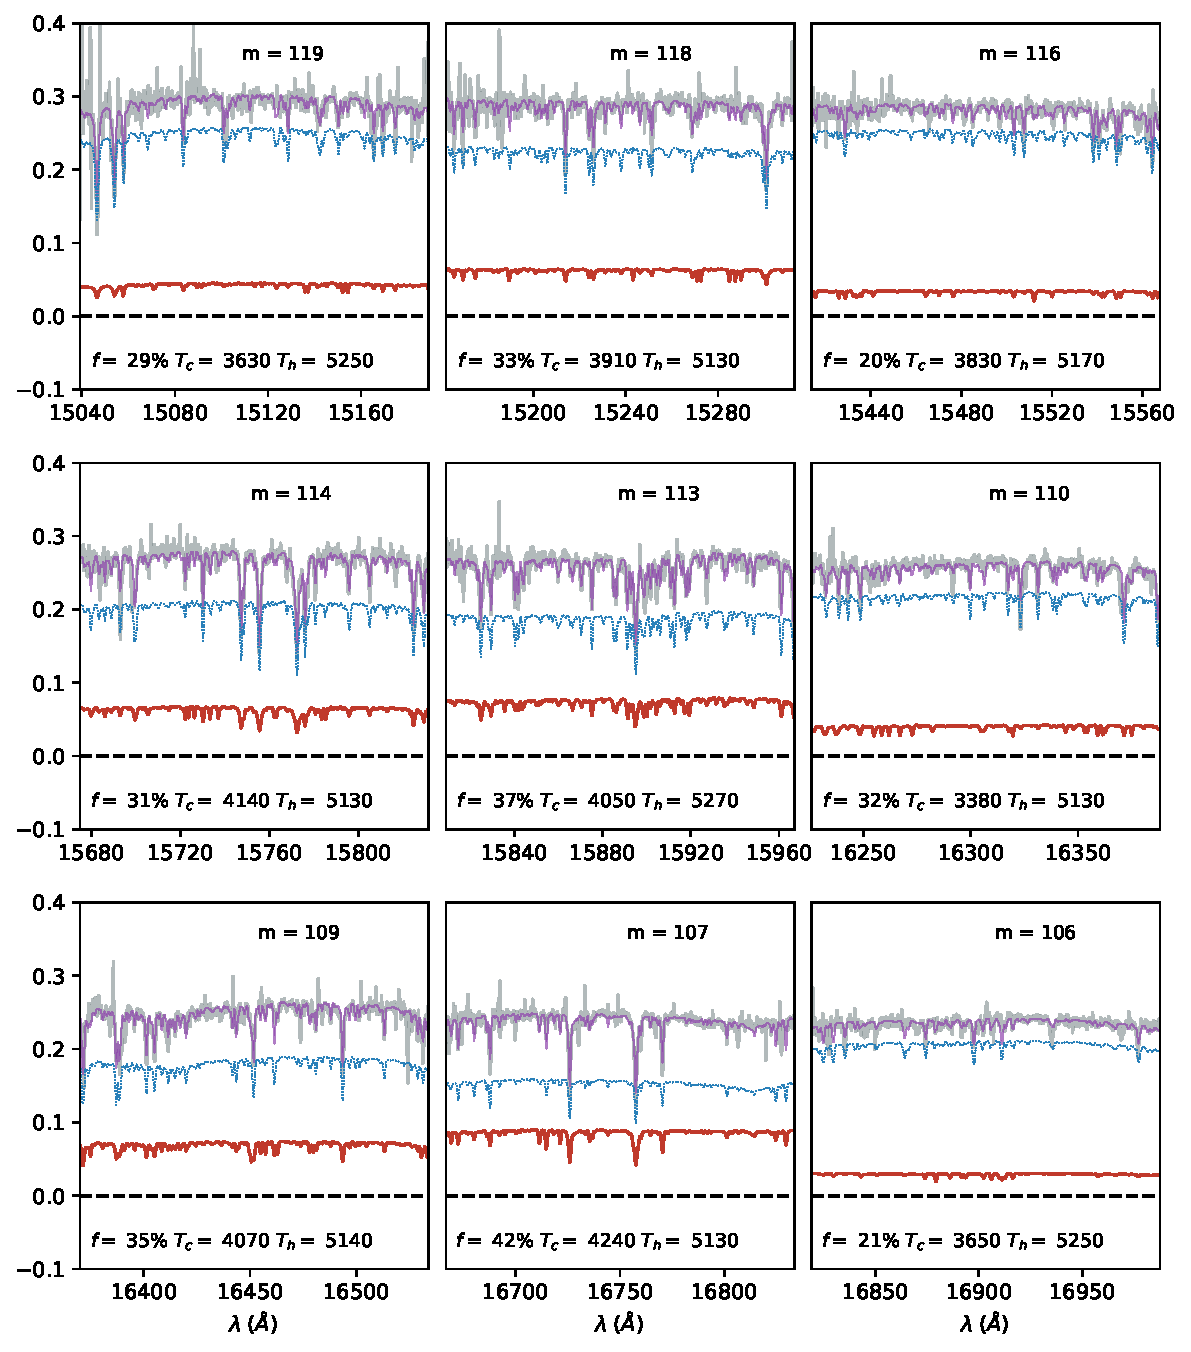
\includegraphics[width=0.98\textwidth]{figures/H_band_spectra_3x3.pdf}
 \caption{Nine $H-$band IGRINS spectral orders with probabilistic spectral decomposition.}
 \label{fig:IGRINS_spectra3x3}
\end{figure*}

\subsubsection{Internal consistency of vsini, $v_z$}
We additionally spot-checked the MCMC posteriors with posterior predictive checks... XX

\item Analysis of near-IR flux contribution from binary companion
\begin{itemize}
  \item Limits on companion types
\end{itemize}
\end{itemize}

\section{Results}

Using the \texttt{Starfish} spectral inference results we investigate the relationship between spot temperature and filling factor. In Figure~\ref{fig:tspot_fillingfactor3x3} we show 2-dimensional distributions of filling factor and spot temperature of the last 200 samples for the nine orders with accepted fits. Similar trends between spot temperature and filling factor appear across most of the orders. Across all nine orders, the median filling factor value is 32\% with a standard deviation of 7\%, with a corresponding spot temperature of $4000 \pm 200$ K. The ambient photosphere temperature associated with this spot signature is $5200\pm25$ K. This is similar to the optical spectroscopic temperature of 5000 K determined by \citet{mathieu03}, which is expected as the optical spectrum will have less significant spot signatures than the IGRINS spectrum in the NIR.

From the 4-year light curve of S1063 (REF LIGHT CURVE FIGURE) we determine that the IGRINS spectrum was observed at a local maximum in the stellar variability, but this flux was approximately 7\% below the global maximum over the four year period covered by ASAS-SN and \textit{K2}. From a first-order interpretation of light curve amplitudes, minimum light corresponds to the largest star spot coverage while maximum light corresponds to the least star spot coverage, although these assumptions are complicated by the possibility of spot evolution \citep{basri18}. Assuming non-emitting spots, the stellar surface must be at least 7\% covered at the time of the IGRINS observation to account for the overall suppression in the maximum flux. If we adopt an ambient photosphere temperature of 5200 K and a spot temperature of 4000 K, the spot coverage would have to be 10\% to account for the flux suppression. At the time of observation, these spectral inference results show that the spot coverage was actually 32\%. This suggests that at the 4-year light curve maximum of S1063, the spot coverage was still around 20\% and definitely not an unspotted star. As seen in Figure LIGHT CURVE, the absolute light curve minimum (occuring at HJD **SOME DATE HERE**) was approximately 13\% lower than the flux at the time of observation. We conclude that the maximum spot filling factor at that time was closer to 50\%.

The time average spot coverage fraction is AMOUNT over the four years, and with that we can calculate the time averaged effective temperature...

(UPDATE THIS WITH TIME AVERAGED SPOT NUMBERS) The presence of spots impacts the effective temperature of S1063. Taking into account both temperature components, we calculate the effective temperature using
\begin{equation}
T_{\textrm{eff}}^4 = f_{\textrm{spot}} T_{\textrm{spot}}^4 + (1 -f_{\textrm{spot}}) T_{\textrm{ambient}}^4 .
\end{equation}
This results in an updated effective temperature for S1063 of $4900\pm125$ K.



\begin{itemize}
\item We MEASURE spots in spectra
\begin{itemize}
  \item S1063 has $32 \pm 7$\% coverage fraction of spots with Tspot $4000\pm200$ K based on IGRINS + Starfish
  \item Revised effective temperature using both temperature components $[f_{\textrm{spot}} * T_{\textrm{spot}}^4 + (1 -f_{\textrm{spot}}) * T_{\textrm{ambient}}^4] = T_{\textrm{eff}}^4$

  \item *bonus* Rsini
\end{itemize}
\item IGRINS observations occurred at maximum of lightcurve, so total spot coverage is even greater
\item *bonus* total spot filling factor estimate given light curve magnitude
\item FIGURE: $T_{spot}$ versus $f_{spot}$ plot


 \begin{figure*}[h]
   \centering
   \begin{tabular}{ccc}
     \subfloat{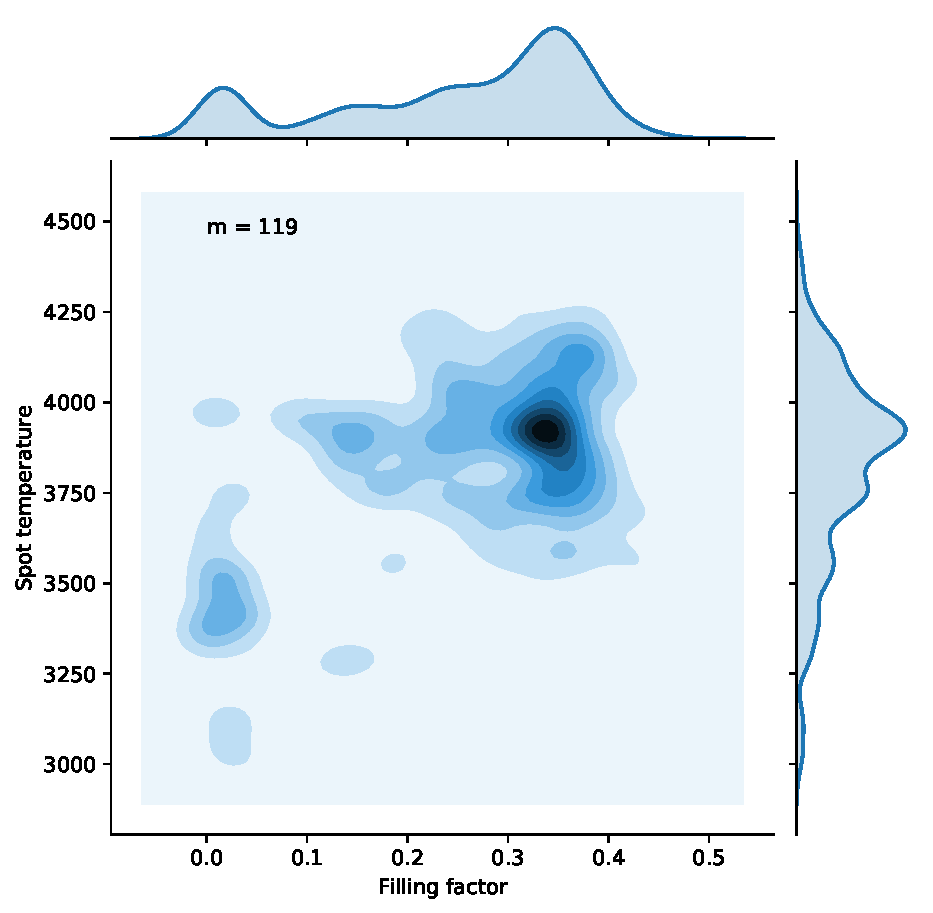
\includegraphics[width=2in]{figures/H_band_Tspot_fillingfactor_m119.pdf}} &
     \subfloat{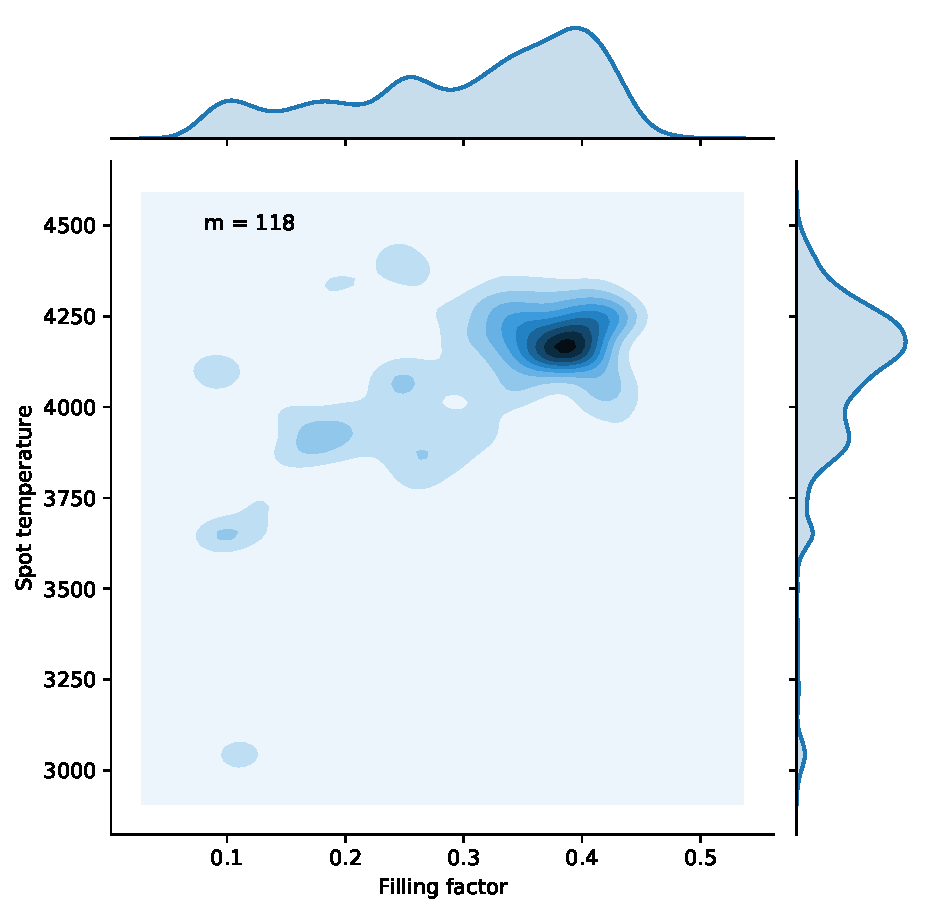
\includegraphics[width=2in]{figures/H_band_Tspot_fillingfactor_m118.pdf}} &
     \subfloat{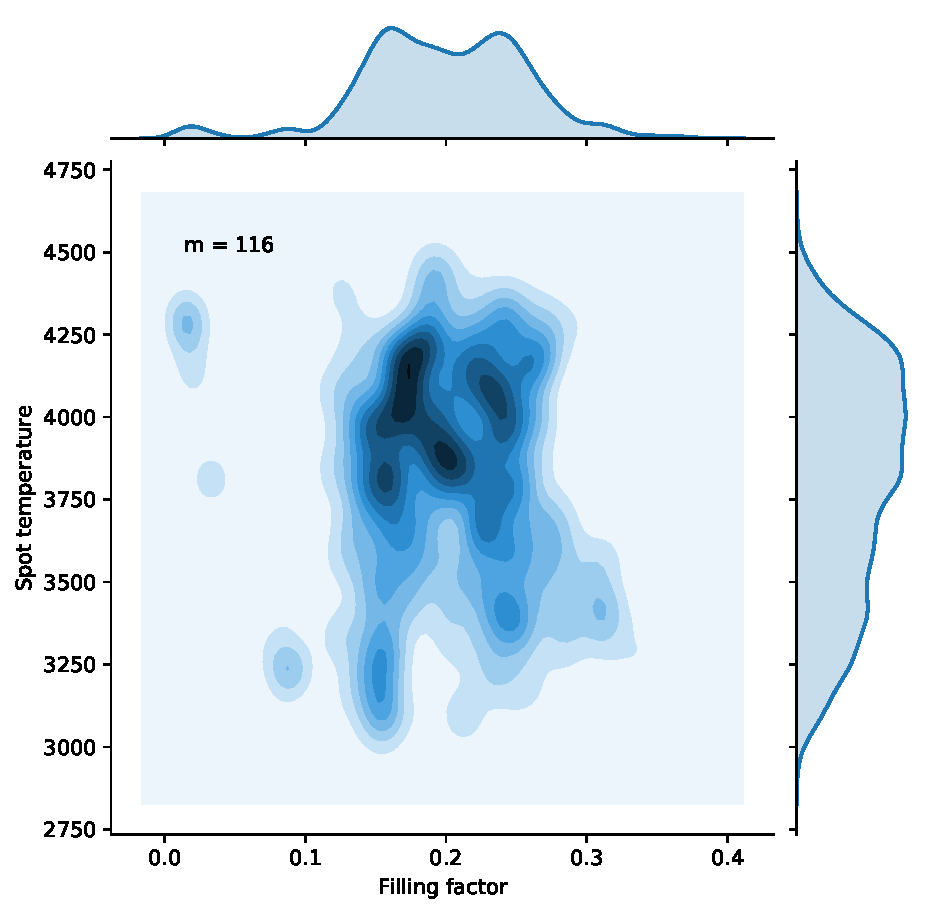
\includegraphics[width=2in]{figures/H_band_Tspot_fillingfactor_m116.pdf}} \\
     \subfloat{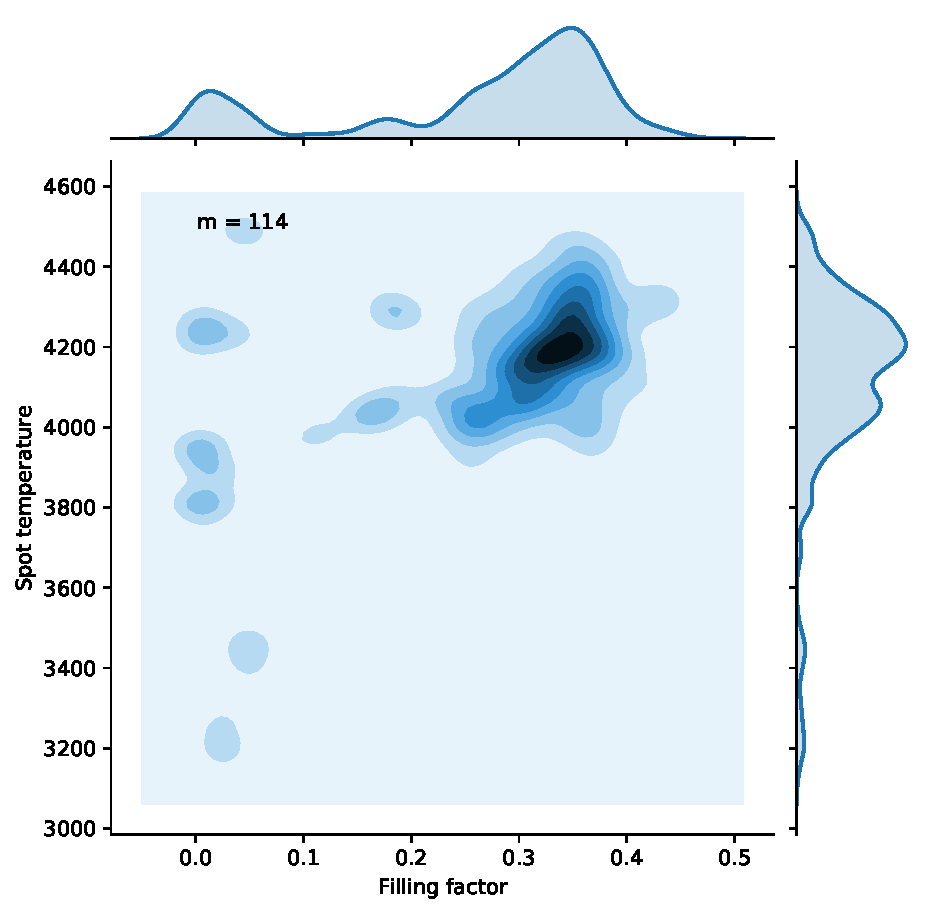
\includegraphics[width=2in]{figures/H_band_Tspot_fillingfactor_m114.pdf}} &
     \subfloat{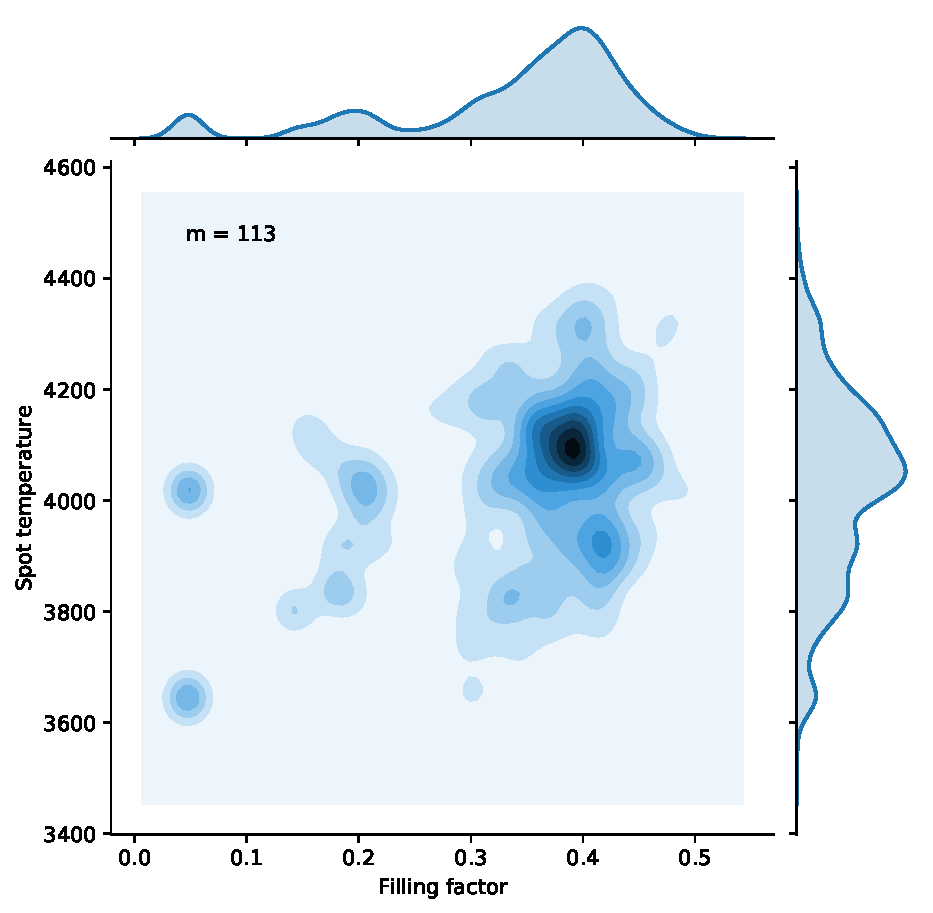
\includegraphics[width=2in]{figures/H_band_Tspot_fillingfactor_m113.pdf}} &
     \subfloat{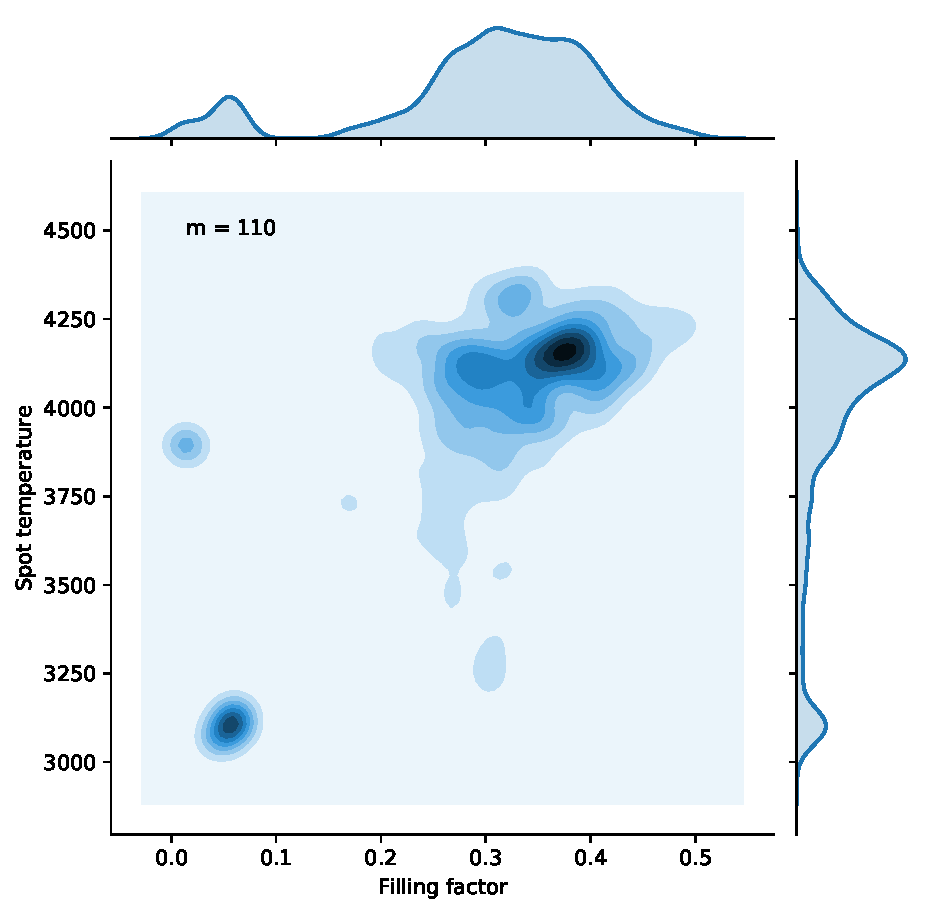
\includegraphics[width=2in]{figures/H_band_Tspot_fillingfactor_m110.pdf}} \\
     \subfloat{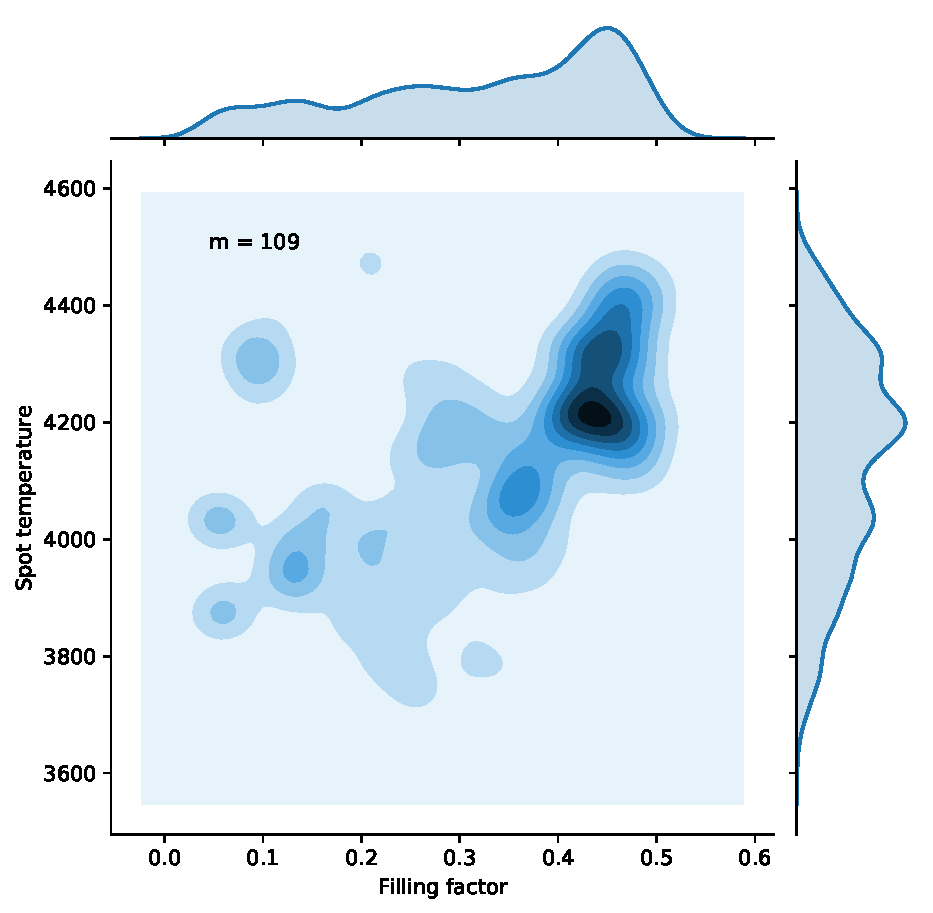
\includegraphics[width=2in]{figures/H_band_Tspot_fillingfactor_m109.pdf}} &
     \subfloat{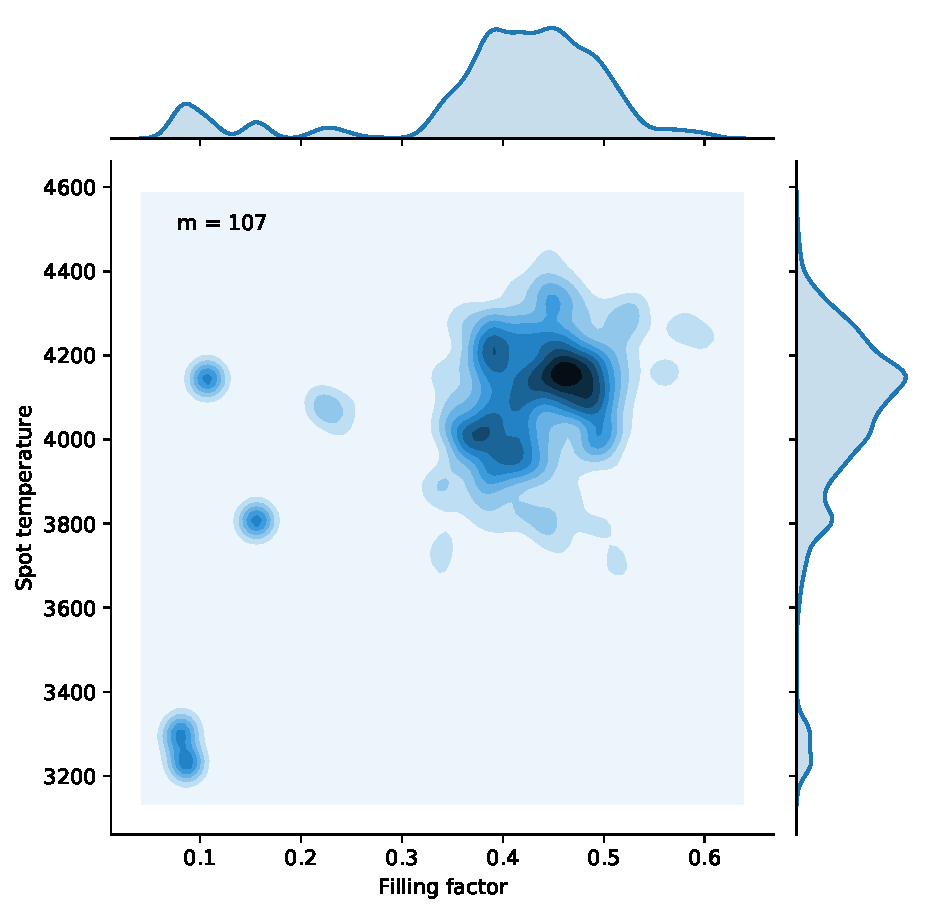
\includegraphics[width=2in]{figures/H_band_Tspot_fillingfactor_m107.pdf}} &
     \subfloat{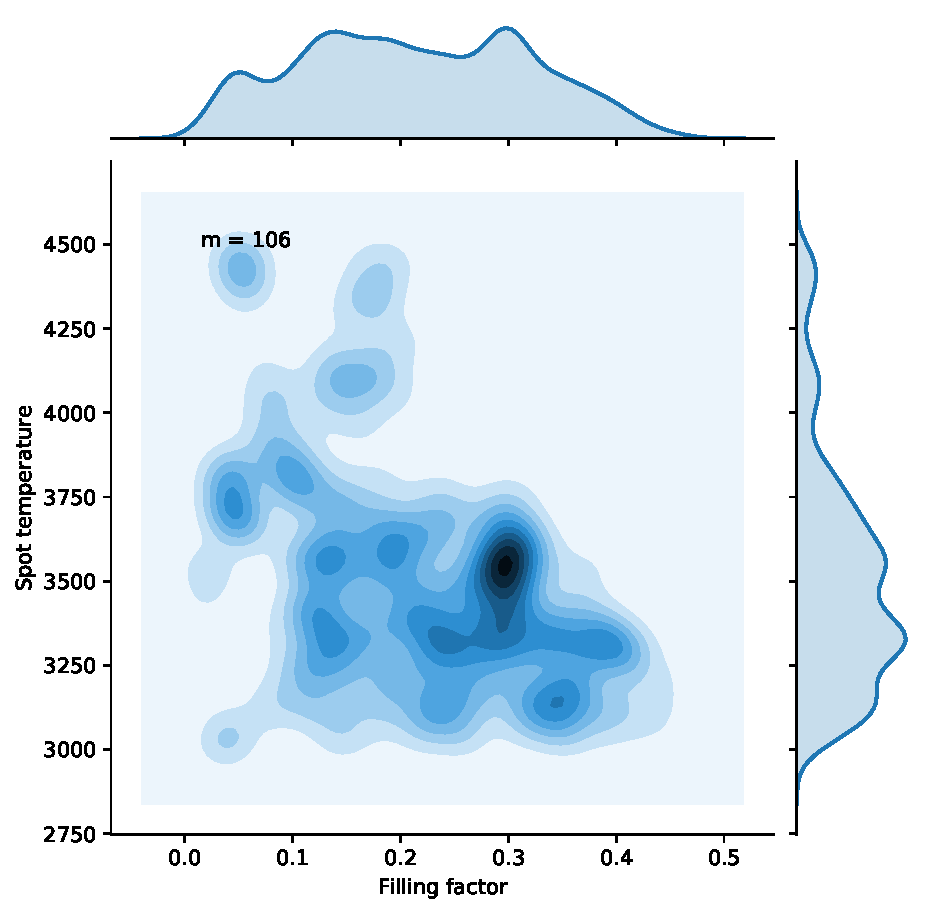
\includegraphics[width=2in]{figures/H_band_Tspot_fillingfactor_m106.pdf}}
   \end{tabular}
 \caption{2-dimensional distributions of filling factor and spot temperature for the nine accepted IGRINS orders for S1063. The median filling factor across these nine orders is $32 \pm 7$\% with a spot temperature of $4000\pm200$ K. As the IGRINS spectrum was observed near maximum light, these show a lower limit on the total spot coverage fraction. }
 \label{fig:tspot_fillingfactor3x3}
 \end{figure*}

\item What coverage fraction would we have measured across the rotational phase?
\end{itemize}

\section{Discussion}


The spot coverage fraction measured here is consistent with the range of spot coverage seen on RS CVn of 30--40\% from measuring TiO band strength \citep{oneal96, oneal98, oneal04} and Doppler imaging \citep{hackman12}. The similar spot coverage fraction on S1063 is further evidence that this sub-subgiant and likely other sub-subgiants have high magnetic activity.

In the absence of this spectral inference technique one could assume the \textit{K2} C5 light curve maximum corresponded to zero spot presence with the light curve amplitude change implying a maximum spot coverage of 7--10\%. This provides a fundamentally different view of the star ...

\begin{itemize}
\item Spot coverage is consistent with formation theories
\item Conceivable geometries with circumpolar active longitudes, or migrating active latitudes
\item Biases introduced if we assume a spot-free model
\begin{itemize}
  \item Where does subsub sit in a new HR diagram? (new Somers models)
  \item *bonus* FIGURE: PMS HR diagram with new Somers tracks
  \item Spot impact on SED fits
\end{itemize}
\end{itemize}

\section{Conclusions}

Reiteration here.

\clearpage
\pagebreak


\appendix

\section{Are starspots confusing?}
\label{methods-details}

Short answer: no!

\acknowledgements

%ADS
We thank ADS!

%IGRINS
This work used the Immersion Grating Infrared Spectrometer(IGRINS) that was developed under a collaboration between the University of Texas at Austin and the Korea Astronomy and Space Science Institute (KASI) with the financial support of the US National Science Foundation under grant AST-1229522, of the University of Texas at Austin, and of the Korean GMT Project of KASI.

%Kepler
This paper includes data collected by the Kepler mission. Funding for the Kepler mission is provided by the NASA Science Mission directorate.

% MAST
Some/all of the data presented in this paper were obtained from the Mikulski Archive for Space Telescopes (MAST). STScI is operated by the Association of Universities for Research in Astronomy, Inc., under NASA contract NAS5-26555.

%gaia
This work has made use of data from the European Space Agency (ESA) mission
{\it Gaia} (\url{https://www.cosmos.esa.int/gaia}), processed by the {\it Gaia}
Data Processing and Analysis Consortium (DPAC,
\url{https://www.cosmos.esa.int/web/gaia/dpac/consortium}). Funding for the DPAC
has been provided by national institutions, in particular the institutions
participating in the {\it Gaia} Multilateral Agreement.


{\it Facilities:} \facility{Smith (IGRINS)}, \facility{AAVSO}, \facility{INTEGRAL (OMC)}, \facility{ASAS}, \facility{Gaia}

{\it Software: }
 \project{pandas} \citep{mckinney10},
 \project{emcee} \citep{foreman13},
 \project{matplotlib} \citep{hunter07},
 \project{numpy} \citep{vanderwalt11},
 \project{scipy} \citep{jones01},
 \project{ipython} \citep{perez07},
 \project{gatspy} \citep{JakeVanderplas2015},
 \project{starfish} \citep{czekala15},
 \project{seaborn} \citep{waskom14}
%\software{%
% \project{pandas} \citep{mckinney10}
%    \project{emcee} \citep{foreman13},
% \project{matplotlib} \citep{hunter07},
% \project{numpy} \citep{vanderwalt11},
% \project{scipy} \citep{jones01},
% \project{ipython} \citep{perez07},
% \project{gatspy} \citep{JakeVanderplas2015},
% \project{starfish} \citep{czekala15}}.

\clearpage

\bibliographystyle{apj}
\bibliography{ms}

\end{document}
